\documentclass[10pt,letterpaper,subeqn]{beamer}
\setbeamertemplate{navigation symbols}{}
\usefonttheme{serif}
\usecolortheme{orchid}



\usepackage[english]{babel}
\selectlanguage{english}
\usepackage{bm}
\usepackage{booktabs}
\usepackage{color}
\usepackage[update,prepend]{epstopdf}
\usepackage{framed}
\usepackage{fleqn}
\usepackage{graphics}
\usepackage{hyperref}
\usepackage[utf8]{inputenc}
%\usepackage{pgf,tikz}
%\usepackage{pgfplots}
\usepackage{setspace}
\usepackage{textcomp}
\usepackage{wrapfig}
\usepackage{multirow}
\usepackage{caption}
\usepackage{subcaption}
%\usepackage[capposition=top]{floatrow}
\setbeamertemplate{caption}[numbered]

%\usetikzlibrary{decorations}



%%\usepackage{amsmath}
%%\usepackage{amssymb}
%%\usepackage{appendix}
%%\usepackage{blindtext}
%%\usepackage{breqn}
%%\usepackage{caption}
%%\usepackage{color}
%%\pagecolor{white}
%%\usepackage{dcolumn}
%%\usepackage{epsfig}
%%
%%\usepackage{framed}
%\usepackage[utf8]{inputenc}
%%\usepackage{pdfpages}
%\usepackage{pgf,tikz}
%\usepackage{pgfplots}
%\usepackage{rotating}
%%
%\usepackage{url}
%%



\title{The Twin Instrument and The Fertility-Investment Trade-off}
\author{Sonia Bhalotra\inst{1} \and Damian Clarke\inst{2}}
\institute{\inst{1} University of Essex \and \inst{2} University of Oxford}
\date{June 2014}



\begin{document}


\begin{frame}
\titlepage
\end{frame}


\section{Motivation}
\frame{\frametitle{The Quantity--Quality Tradeoff}
\begin{itemize}
 \item Cross-sectional data within and across regions suggests that children from larger families have weaker educational outcomes, e.g. Hanushek 1992, Blake 1989.
 \item This empirical regularity is often attributed to a quantity-quality (QQ) tradeoff in parental investments: Becker 1960, Becker and Lewis 1973, Becker and Tomes 1976.
 \item Child quality and child quantity enter multiplicatively in the budget constraint. It follows that (Galor 2012)- 
\begin{itemize}
 \item Exogenous reductions in the price of quality raise the shadow price of having more children.
 \item \textcolor{red}{Exogenous reductions in the price of quantity (of children) reduce the marginal cost of investing in quality}
\end{itemize}
\end{itemize}
}

\frame{\frametitle{Relevance}
\begin{itemize}
\item The negative reinforcing mechanism between q \& q plays a central role in macro-growth models with endogenous fertility.
\begin{itemize}
\item Becker and Barro 1988, Becker et al. 1990, Moav 2005.
\end{itemize}
\item Many countries have implemented aggressive fertility control policies, e.g. China, India, Mexico, Indonesia.
\begin{itemize}
\item Echoes Malthus.
\item Idea is that this is good for human capital and growth.
\end{itemize}
\end{itemize}
}

\frame{\frametitle{Evidence}
\begin{itemize}
\item \textcolor{blue}{Limited causal evidence}
\item \textcolor{blue}{Limitations of causal evidence}
\item \textcolor{blue}{Overall, some doubt that a QQ tradeoff exists}
\item \textcolor{blue}{Using twins as an instrument}, Black et al. 2005 (Norway) and Angrist et al. 2010 (Israel) find no evidence of a relationship between fertility and schooling.
\begin{itemize}
\item Some evidence of a trade off using other quality indicators: Juhn et. al. 2013, Conley and Glauber 2006, Caceres-Delpiano 2006.
\end{itemize}
\item \textcolor{blue}{Using change in price of quality}, recent studies find a trade off: Bleakley 2007, Bhalotra and Venkataramani 2012, Aaranson et al. 2013 
\end{itemize}
}

\frame{\frametitle{Our Contributions}
We argue that an underlying QQ tradeoff may be obscured.
\vspace{6mm}
\begin{itemize}
\item \textcolor{blue}{Twin birth is not exogenous (even if twin conception is)}
\begin{itemize}
\item In particular, the health of the mother is a potential omitted variable in previous studies.
\item Existing estimates are biased, inconsistent
\item We show that this is the case in a wide range of contexts (Chile, USA, Scotland, DHS\ldots)
\end{itemize}
\item We assemble a large micro-data sample for developing countries and assess whether the tradeoff is evident in \textcolor{blue}{poorer} countries.
\begin{itemize}
\item Previous work has argued that credit constraints on investment in child quality may not be binding in richer countries
\end{itemize}
\end{itemize}
}

\section{Motivation}
\frame{\frametitle{IV Procedure}
\begin{equation}
\label{TWINeqn:secondstage}
educ_{ij}=\beta_0+\beta_1 fert_{j} + \bm{X}\bm{\beta}_2+u_{ij}.
\end{equation}
\begin{equation}
\label{TWINeqn:firststage}
fert_{j}=\alpha_0+\alpha_1 twins_{j}+\bm{X}\bm{\alpha}_2+\nu_{j},
\end{equation}
\vspace{2mm}
And so assuming:
\[
E[fert_j\cdot u_{ij}] \neq 0, \ E[twins_j\cdot u_{ij}] = 0
\]
\vspace{6mm}
\begin{itemize}
\item Previous studies assume twin incidence is a valid instrument.
\item A key concern is whether IV estimates are precise enough to be informative (and distinguishable from OLS estimates): Angrist et al.\ 2010.
\end{itemize}
}

\frame{\frametitle{Twin Exogeneity}
\begin{enumerate}
\item \textcolor{blue}{Refurbish $\bm{X}$}.  Ours is the first attempt to condition on (partial indicators) of mother's health
\item \textcolor{blue}{Estimate bounds} on qq-parameter when twin instrument is almost but not exactly exogenous.
\end{enumerate}
Thereby assess possibility that there is a QQ tradeoff, obscured in recent studies by bias associated with assuming twin exogeneity.
}

\frame{\frametitle{Twin Exogeneity}
\begin{itemize}
\item Assuming additive separability of $u_{ij}$: $u_{ij}=u_{ij}^S+u_{ij}^H+u_{ij}^*$
\item `typical estimate': 
\end{itemize}
\[
\hat\beta_1^{IV} = \beta_1 + P\lim \frac{1}{N}twin_ju^S_{ij} + 
P\lim \frac{1}{N}twin_ju^H_{ij} + P\lim \frac{1}{N}twin_ju^*_{ij}
\]
\begin{itemize}
\item By including elements $S$ and $H$ in $\bm{X}$, this becomes:
\end{itemize}
\[
\hat\beta_1^{IV,S+H} = \beta_1 + P\lim N^{-1}twin_ju^*_{ij},
\]
\begin{itemize}
\item where it is likely that $\hat\beta_1^{IV}>\hat\beta_1^{IV,H}>\hat\beta_1^{IV,S+H}>\beta_1.$
\end{itemize}
}

%\frame{\frametitle{Innovation 2: Desired Fertility}
%Use information on \textcolor{blue}{twin parity relative to target fertility}.
%\vspace{5mm}
%\begin{itemize}
%\item The Wald estimator is the weighted average causal response for people from families induced by an instrum%ent to go from having fewer than j to at least j children, weighted over j by the probability of crossing this %threshold. 
%\item The denominator normalizing the weights is the Wald first stage.
%\item Individuals with $C_{1i} \geq j \geq C_{0i}$ are compliers a la Angirst, Imbens, Rubin 1996. Differences %in 1st stage coefficients indicate differences in probability of compliance across groups.
%\end{itemize}
%}


\section{Data}
\frame{\frametitle{Data and Context}
\begin{itemize}
\item Comparable cross-country micro-data for developing countries from the Demographic and Health Surveys
\begin{itemize}
\item Complete fertility histories, subjective reports of desired fertility, indicators of maternal health, maternal education and child education.
\end{itemize}
\item Merge all surveys between 1991 and 2013: sample of 2,721,619 children from 68 countries
\begin{itemize}
\item Large sample useful given twin are rare (sample mean 1.89\%)
\item Outcome: schooling (z-score). Retain children age 6-17 at survey date.
\item Birth cohorts 1971-2012
\end{itemize}
\item Countries classified as low vs middle income by the World Bank
\begin{itemize}
\item Women in poor countries under-nourished and less able to take twin conceptions to term. Higher desired fertility, twins are less likely than otherwise to take actual over desired fertility. Low schooling.
\end{itemize}
\end{itemize}
}

\frame{\frametitle{Data and Context}
\begin{itemize}
\item \textcolor{red}{Effects of twins at parity $j$ on outcomes for births $j-1$ and before} (as in Black et al. 2005). 
\begin{itemize}
\item Predictions are for \textcolor{red}{infra-marginal} children.
\end{itemize}
\item Nomenclature: ``2+ sample'' - Firstborn subjects in families with at least two births (allowing that a birth may be twin). 
\begin{itemize}
\item Instrument with twins at second birth
\end{itemize}
\item ``3+ sample'': First and second born subjects in families with at least three births 
\begin{itemize}
\item Instrument with twins at third birth
\end{itemize}
\item And simiarly for 4+.  Twin subjects are generally dropped.
\end{itemize}
}

\frame{
\begin{itemize}
\item By restricting to \textcolor{blue}{families with at least $j$ births} on average we ensure that preferences over family size are the same in the families with twins at the $jth$ birth and those with singleton births
\item By restricting the sample to \textcolor{blue}{children born before birth $j$}, we avoid selection problems that arise because families who choose to have another child after a twin birth may differ from families who choose to have another child after a singleton birth.
\end{itemize}
}

\section{Twin Births Are Correlated With Mother Characteristics}
\frame{\frametitle{Mother's Health}
\begin{itemize}
 \item Evidence from the cross-country microdata sample shows that indicators of the health of the mother influence child birth-weight, survival and growth (stunting): Bhalotra and Rawlings (2013). 
 \item This makes it plausible that mother’s health influences foetal survival.
\begin{itemize}
 \item A standard deviation decrease in mother's height or BMI raises the risk of poor child health (birth-weight, mortality, stunting) by between 5 and 10 per cent, depending on the measure.
\item The risks of low birth weight and neonatal mortality are higher by 5.7\% and 16.9\% of their mean rates amongst mothers who have anemia relative to mothers who do not.
\end{itemize}
\end{itemize}
}

\frame{\frametitle{Mother's Health}
\begin{itemize}
\item \textcolor{red}{No previous evidence (or discussion) of maternal health being a predictor of twin births.}
\item But, recognised that maternal health and behaviours affects a large number of other birth and longer term outcomes (Mazumder and Seeskin, 2014; Black et al.\ 2014; Almond et al.\ 2011; Barker 1995).
\item And evidence from medical literature (Li et al.\ 2003, Hall 2003) that Pr(twinning) increases with age, weight and height (mediated by follicle stimulating hormone) 
\end{itemize}
}



\frame{\frametitle{Investigating Exogeneity of Twins -- 1}
\begin{equation}
\label{TWINeqn:twinreg}
P(twin_{j})=\gamma_0 + \bm{X}\bm{\gamma}_1 + \bm{S}\bm{\gamma}_2
                  + \bm{H}\bm{\gamma}_3 + \varepsilon_{j}.
\end{equation}
\begin{itemize}
\item Equivalent: \textcolor{blue}{Test of balance} of characteristics (X) between mothers who have twins and mothers who do not
\item $\bm{X}, \bm{S}$ and $\bm{H}$ are mother characteristics potentially correlated with child quality: age, wealth, education, height, BMI, antenatal care, smoking/drinking/drugs during pregnancy.
\item If twin birth is a random event $\bm{\gamma_1}=\bm{\gamma_2}=\bm{\gamma_3}=0$
\item \textcolor{red}{Can typically condition on only a subset of predictors $X$}
\end{itemize}
}

\frame{\frametitle{Investigating Exogeneity of Twins -- 2: Women who have twin births are healthier}
\[Quality_{t-k}=\alpha twins_{t}+\bm{X}\delta + \varepsilon \]
\vspace{5mm}
\begin{itemize}
\item Compare child quality in families with and without twins at parity $p$ for children born at earlier parities. 
\item But use a measure of quality (investment) that is necessarily determined before twins occur: infant mortality.
\item If twins occur randomly, $\alpha=0$
\end{itemize}
}

\frame{
\begin{table}[htbp]\centering
\def\sym#1{\ifmmode^{#1}\else\(^{#1}\)\fi}
\caption{Test of Balance of Observables: Twins versus Non-twins \label{TWINtab:comp}}
\vspace{5mm}\begin{tabular}{l*{1}{ccc}}
\toprule\toprule & Non-Twin & Twin & Diff.\\
                    &        Family&        Family&      (Diff. SE)         \\
\midrule
Total Fertilty      &       4.460&       6.787&      -2.327\sym{***}\\
                    &            &            &    (0.0255)         \\
Desired Fertility   &       4.451&       5.566&      -1.116\sym{***}\\
                    &            &            &    (0.0312)         \\
Age First Birth     &       19.15&       18.98&       0.170\sym{***}\\
                    &            &            &    (0.0424)         \\
Mother's Education  &       4.269&       3.351&       0.918\sym{***}\\
                    &            &            &    (0.0523)         \\
Father's Education  &       5.510&       4.710&       0.800\sym{***}\\
                    &            &            &    (0.0584)         \\
Mother's Height     &       156.1&       157.8&      -1.716\sym{***}\\
                    &            &            &    (0.0839)         \\
Pr(BMI $<$ 18.5)    &       0.120&      0.0937&      0.0265\sym{***}\\
                    &            &            &   (0.00382)         \\
Number of Antenatal Checks&       3.901&       3.815&      0.0860\sym{*}  \\
                    &            &            &    (0.0374)         \\
Prenatal care (doctor)&       0.313&       0.211&       0.102\sym{***}\\
                    &            &            &   (0.00544)         \\
Prenatal care (nurse)&       0.452&       0.521&     -0.0690\sym{***}\\
                    &            &            &   (0.00588)         \\
Prenatal care (none)&       0.193&       0.183&     0.00979\sym{*}  \\
                    &            &            &   (0.00466)         \\
Mother's Age        &       25.53&       27.61&      -2.077\sym{***}\\
                    &            &            &    (0.0565)         \\
Child Mortality     &      0.0102&      0.0255&     -0.0153\sym{***}\\
                    &            &            &  (0.000912)         \\
Infant Mortality    &     0.00580&      0.0170&     -0.0112\sym{***}\\
                    &            &            &  (0.000606)         \\
Wealth Quintile 1   &       0.259&       0.274&     -0.0154\sym{**} \\
                    &            &            &   (0.00518)         \\
Wealth Quintile 2   &       0.220&       0.227&    -0.00691         \\
                    &            &            &   (0.00490)         \\
Wealth Quintile 3   &       0.198&       0.201&    -0.00351         \\
                    &            &            &   (0.00471)         \\
Wealth Quintile 4   &       0.176&       0.175&    0.000653         \\
                    &            &            &   (0.00450)         \\
Wealth Quintile 5   &       0.148&       0.123&      0.0252\sym{***}\\
                    &            &            &   (0.00418)         \\
\midrule\midrule


\multicolumn{4}{p{10.4cm}}{\begin{footnotesize}\textsc{Notes:} Education measured in years, mother's height in centimetres, and BMI is weight in kilograms over height in metres squared.  Diff. SE is calculated using a two-tailed t-test. $^{*}$p$<$0.1; $^{**}$p$<$0.05; $^{***}$p$<$0.01\end{footnotesize}}
\\\bottomrule\normalsize\end{tabular}\end{table} 

}

\frame{
\begin{landscape}\begin{table}[htpb!] 
\caption{Probability of Giving Birth to Twins} \label{TWINtab:twinreg1} 
\begin{center}\begin{tabular}{lcccccc} \toprule \toprule 
&(1)&(2)&(3)&(4)&(5)&(6)\\
Twin$\times$100&All&\multicolumn{2}{c}{Income}&\multicolumn{2}{c}{Time}&Prenatal\\
 \cmidrule(r){3-4} \cmidrule(r){5-6} 
&&Low inc&Middle inc&1990-2013&1972-1989&\\\midrule
\begin{footnotesize}\end{footnotesize}&\begin{footnotesize}\end{footnotesize}&\begin{footnotesize}\end{footnotesize}&\begin{footnotesize}\end{footnotesize}&\begin{footnotesize}\end{footnotesize}&\begin{footnotesize}\end{footnotesize}&\begin{footnotesize}\end{footnotesize}\\
Age&0.491***&0.489***&0.498***&0.587***&0.168***&0.632***\\
&(0.026)&(0.033)&(0.045)&(0.030)&(0.064)&(0.040)\\
Age Squared&-0.006***&-0.006***&-0.007***&-0.008***&-0.000&-0.009***\\
&(0.000)&(0.001)&(0.001)&(0.001)&(0.001)&(0.001)\\
Age First Birth&-0.051***&-0.082***&-0.002&-0.050***&-0.051***&-0.041***\\
&(0.008)&(0.010)&(0.013)&(0.009)&(0.015)&(0.013)\\
Education (years)&0.027*&0.065***&-0.008&0.044**&-0.008&-0.071**\\
&(0.016)&(0.021)&(0.027)&(0.019)&(0.028)&(0.028)\\
Education squared&-0.001&-0.005**&0.001&-0.002&0.002&0.003\\
&(0.001)&(0.002)&(0.002)&(0.001)&(0.002)&(0.002)\\
Height&0.057***&0.056***&0.058***&0.063***&0.038***&0.059***\\
&(0.004)&(0.005)&(0.006)&(0.005)&(0.007)&(0.007)\\
BMI&0.050***&0.059***&0.043***&0.046***&0.056***&0.045***\\
&(0.006)&(0.008)&(0.008)&(0.007)&(0.009)&(0.011)\\
Prenatal (Doctor)&&&&&&0.917***\\
&&&&&&(0.129)\\
Prenatal (Nurse)&&&&&&0.076\\
&&&&&&(0.109)\\
Prenatal (None)&&&&&&-0.479***\\
&&&&&&(0.133)\\
&&&&&&\\R-squared&0.01&0.01&0.01&0.01&0.00&0.01\\
Observations &2271948&1430703&841245&1660253&611695&624990\\
\hline\hline\multicolumn{7}{p{14.3cm}}{\begin{footnotesize}\textsc{Notes:} All specifications include a full set of year of birth and  country dummies, and are estimated as linear probability models.  Twin is multiplied by 100 for presentation.  Height is measured in cm  and BMI is weight in kg divided by height in metres squared. l  Prenatal care variables are only recoreded for recent births.  As  such, column (6) is estimated only for that subset of births where  these observations are made.
$^{*}$p$<$0.1; $^{**}$p$<$0.05; $^{***}$p$<$0.01
 \end{footnotesize}}\\ \hline \normalsize \end{tabular}\end{center}\end{table}\end{landscape} 

}

\frame{\frametitle{Effect Sizes}
Substantial marginal effects of observed indicators of mother’s health on the probability of twin birth (mean=2\%)
\vspace{6mm}
\begin{itemize}
\item A one s.d. change in the height of the mother results in an increase of 0.44\% points (22\% of mean)
\item A one s.d. change in mother’s BMI results in an increase of 0.20\% points (10\% of mean)
\end{itemize}
}

\frame{\frametitle{Is This an Artifact of DHS Data?}
\begin{itemize}
\item We have run similar tests using a number of surveys and administrative data sets:
  \begin{itemize}
  \item DHS (above)
  \item Chile
  \item Scotland
  \item UK
  \item USA
 \end{itemize}
\item Depending upon data availability we include health stocks, behaviour
\item This does not appear to be restricted to poor countries:
\end{itemize}
}

\frame{
\begin{table}[htpb!] 
\caption{Probability of Giving Birth to Twins (Chile)} 
\label{TWINtab:Chile} 
\begin{center}\begin{tabular}{lclc} \toprule \toprule 
&(1)&&\\
Twin$\times$100&&&\\\midrule
\multicolumn{2}{l}{\textsc{Pre-Pregnancy}}&\multicolumn{2}{l}{\textsc{Pregnancy}}\\\begin{footnotesize}\end{footnotesize}&\begin{footnotesize}\end{footnotesize}&\begin{footnotesize}\end{footnotesize}&\begin{footnotesize}\end{footnotesize}\\
Income p.c.&-0.006&Smoked&-0.573\\
&	(0.011)
&&	(0.416)
\\
Income p.c. squared&0.000&Drugs (infrequent)&-0.119\\
&	(0.000)
&&	(1.646)
\\
Secondary Education&0.142&Drugs (frequent)&-1.872***\\
&	(0.300)
&&	(0.344)
\\
Tertiary Education&1.507***&Alcohol (infrequent)&-0.002\\
&	(0.583)
&&	(0.570)
\\
Low Weight&-0.589&Alcohol (frequent)&-1.891***\\
&	(0.471)
&&	(0.290)
\\
Obese&-1.997***&No Check-ups&-1.031\\
&	(0.766)
&&	(0.966)
\\
Mother's Age&0.410***&Hospital Birth&0.939***\\
&	(0.133)
&&	(0.344)
\\
Mother's Age Squared&-0.007***&Diabetes&-0.255\\
&	(0.002)
&&	(0.505)
\\
Indigenous&-1.027***&Depression&0.031\\
&	(0.395)
&&	(0.416)
\\
&&&\\
Observations&14268&R-squared&0.00\\
\midrule\multicolumn{4}{p{11cm}}{\begin{footnotesize}\textsc{Notes:} Data comes from the Encuesta Longitudinal de Primera Infancia (ELPI) from Chile. Education at each level are dummy variables, primary education is the omitted base. Regional controls and child age fixed effects are omitted for clarity. Heteroscedasticity robust standard errors are presented in parenthesis.$^{*}$p$<$0.1; $^{**}$p$<$0.05; $^{***}$p$<$0.01\end{footnotesize}}\\ \hline \normalsize \end{tabular}\end{center}\end{table}

}

\frame{
\begin{table}[htpb!] 
\caption{Probability of Giving Birth to Twins (Scotland)} 
\label{TWINtab:Scotland} 
\begin{center}\begin{tabular}{lclc} \toprule \toprule 
&(1)&&\\
Twin$\times$100&&&\\\midrule
\multicolumn{2}{l}{\textsc{Pre-Pregnancy}}&\multicolumn{2}{l}{\textsc{Pregnancy}}\\\begin{footnotesize}\end{footnotesize}&\begin{footnotesize}\end{footnotesize}&\begin{footnotesize}\end{footnotesize}&\begin{footnotesize}\end{footnotesize}\\
Deprivation Index (Quintile 2)&-1.628**
&Smoker&0.001
\\
&(0.958)
&&(0.669)
\\
Deprivation Index (Quintile 3)&-0.188
&Previous Smoker&1.717**
\\
&(0.967)
&&(0.877)
\\
Deprivation Index (Quintile 4)&-0.421
&Alcohol (1-2 per week)&-4.498*
\\
&(0.934)
&&(1.935)
\\
Deprivation Index (Quintile 5)&-1.132
&Alcohol (3+ per week)&-3.030*
\\
&(0.920)
&&(1.543)
\\
Height&0.306***
&Overweight&-0.092
\\
&(0.044)
&&(0.643)
\\
Married&3.272***
&Obese&1.350**
\\
&(0.878)
&&(0.746)
\\
Age&-0.337
&Diabetes&-0.188
\\
&(0.400)
&&(0.967)
\\
Age Squared&0.020***
&&\\
&(0.007)
&&\\
&&&\\
Observations&193254
&R-squared&0.01\\
\midrule\multicolumn{4}{p{11cm}}{\begin{footnotesize}\textsc{Notes:} Data comes from the ADD NOTE HERE!.$^{*}$p$<$0.1; $^{**}$p$<$0.05; $^{***}$p$<$0.01\end{footnotesize}}\\ \hline \normalsize \end{tabular}\end{center}\end{table}

}

\frame{
 \begin{table}[htpb!] 
\caption{Probability of Giving Birth to Twins (UK)} 
\label{TWINtab:UK} 
\begin{center}
\scalebox{0.6}{
\begin{tabular}{lclc} \toprule \toprule 
&(1)&&\\
Twin$\times$100&&&\\\midrule
\midrule\multicolumn{4}{p{11cm}}{\begin{footnotesize}\textsc{Notes:}$^{*}$p$<$0.1; $^{**}$p$<$0.05; $^{***}$p$<$0.01\end{footnotesize}}\\ \hline \normalsize \end{tabular}}\end{center}\end{table}

}


\frame{\frametitle{USA Birth Records}
In preliminary results from National Vital Statistics System (NVSS) which register all births in USA from 1995-2000 (23.5 million observations):
\vspace{5mm}
\begin{itemize}
\item Education is significantly positively related to having a twin
\item Drinking while pregnant is significantly negatively related to having a twin
\item Smoking while pregnant is significantly negatively related to having a twin
\item Age, race and more previous births are significant predictors
\end{itemize}
}


\frame{\frametitle{Second Test of Exogeneity of Twins: Are mothers who produce twins healthier ex ante?}
\begin{itemize}
\item Comparison of child outcome determined before twins arise across families who do and do not subsequently have a twin birth
\item Results indicate that twin births occur in families with a tendency towards lower infant morality, possibly healthier (or better-off) families.
\end{itemize}
\begin{table}[htpb!]
\caption{Test of hypothesis that women who bear twins have better prior health}\label{TWINtab:IMR}\begin{center}\begin{tabular}{lccc}
\toprule \toprule 
\textsc{Infant Mortality (per 100 births)}& Base & +S\&H & Observations \\ \midrule 
\begin{footnotesize}\end{footnotesize}& 
\begin{footnotesize}\end{footnotesize}& 
\begin{footnotesize}\end{footnotesize}& 
\begin{footnotesize}\end{footnotesize}\\ 
Treated (2+)\hspace{5mm}\hspace{5mm}\hspace{5mm}\hspace{5mm}\hspace{5mm}\hspace{5mm}&-2.065***&-2.110***&503785\\
&(0.212)&(0.213)&\\
Treated (3+)\hspace{5mm}&-4.619***&-4.632***&686931\\
&(0.201)&(0.201)&\\
Treated (4+)&-4.257***&-4.243***&676303\\
&(0.183)&(0.183)&\\
Treated (5+)&-3.353***&-3.324***&587919\\
&(0.183)&(0.183)&\\
\midrule\multicolumn{4}{p{12.1cm}}{\begin{footnotesize}\textsc{Notes:} The sample for these regressions consist of all children who have been entirely exposed to the risk of infant mortality (ie those over 1 year of age). Subsamples 2+, 3+, 4+ and 5+ are generated to allow comparison of children born at similar birth orders.  For a full description of these groups see the the body of the paper or notes to table \ref{TWINtab:IVAll}. Treated=1 refers to children who are born before a twin while Treated=0 refers to children of similar birth orders not born before a twin.  Base and S+H controls are described in table \ref{TWINtab:IVAll}.$^{*}$p$<$0.1; $^{**}$p$<$0.05; $^{***}$p$<$0.01 
\end{footnotesize}} \\ \bottomrule 
\end{tabular}\end{center}\end{table}
}


\section{Descriptive Statistics}
\frame{\frametitle{Trends in Education, Fertility, Fertility Control}
\begin{figure}[htpb!]
\centering
\begin{subfigure}{.5\textwidth}
  \centering
  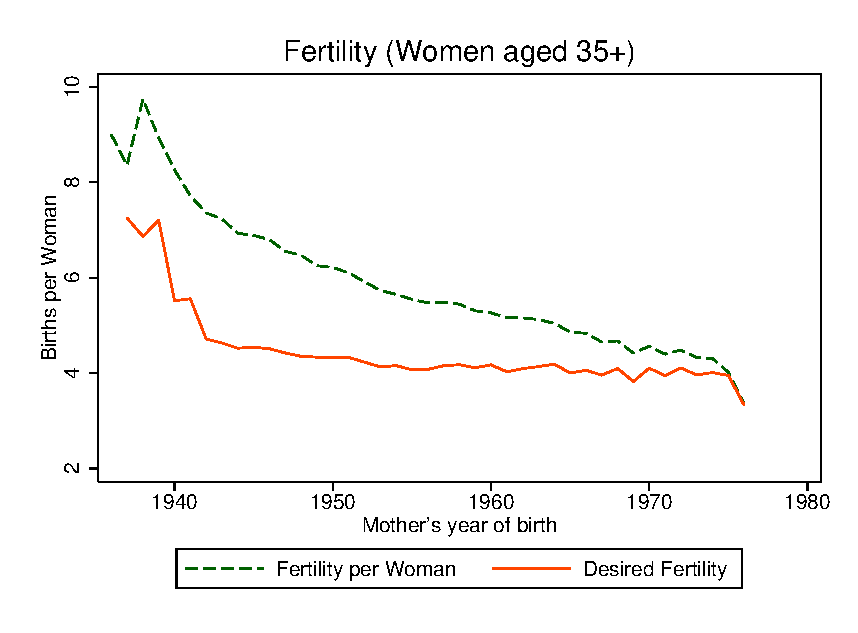
\includegraphics[scale=0.37]{./figures/ferttrend_35_all.eps}
  \caption{Trends in Fertility}
  \label{TWINfig:fertrend}
\end{subfigure}%
\begin{subfigure}{.5\textwidth}
  \centering
  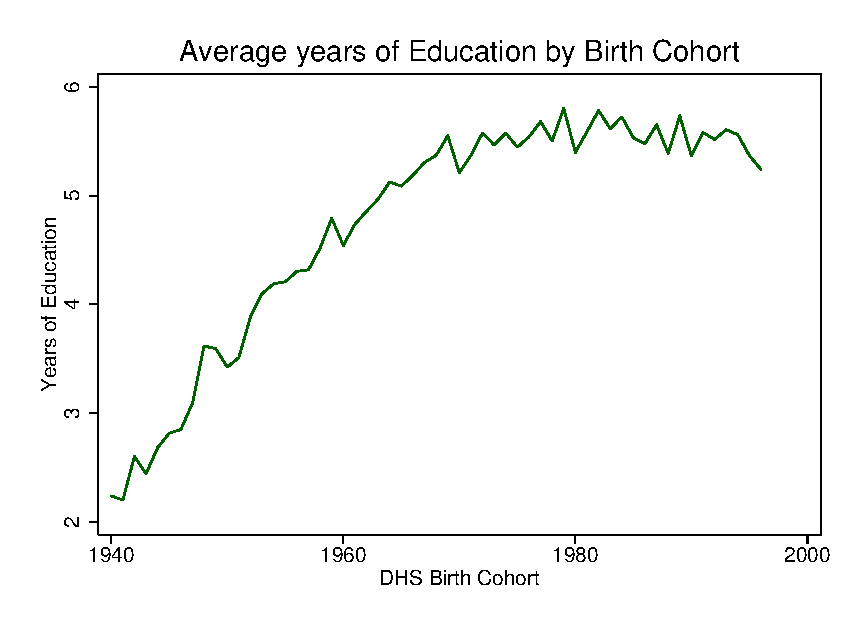
\includegraphics[scale=0.35]{./figures/eductrend_all.eps}
  \caption{Trend in Education}
  \label{TWINfig:eductrend}
\end{subfigure}
\caption{Education and Fertility}
\label{TWINfig:trends}
\footnotesize{Note to figures: Cohorts are made up of all individuals 
from the DHS who are over 35 years (for fertility), and over 15 years (for education).  
In each case the sample is restricted to those who have approximately completed fertility 
and education respectively.}
\end{figure}
}

\frame{
\begin{table}[htpb!]\caption{Summary Statistics} 
\label{TWINtab:sumstats}\begin{center}\scalebox{0.6}{\begin{tabular}{lccccc}
\toprule \toprule 
&\multicolumn{2}{c}{Low Income}&\multicolumn{2}{c}{Middle Income}\\ 
\cmidrule(r){2-3} \cmidrule(r){4-5}
& Single & Twins & Single & Twins & All \\ \midrule 
\textsc{Fertility} & & & & & \\ 
Fertility&3.670&6.093&3.348&5.425&3.609\\
&(2.365)&(2.582)&(2.272)&(2.609)&(2.372)\\
Desired Family Size&4.182&5.296&3.340&4.128&3.892\\
&(2.500)&(2.832)&(2.083)&(2.498)&(2.403)\\
Fraction Twin & \multicolumn{2}{c}{  0.0194}& \multicolumn{2}{c}{  0.0173 } &  0.0185\\
& \multicolumn{2}{c}{(0.1379)}& \multicolumn{2}{c}{(0.1306)} & (0.1348)\\
\textsc{Health of Mother}&&&&&\\ 
Height&155.6&157.7&155.6&157.2&155.7\\
&(7.084)&(6.987)&(6.956)&(6.957)&(7.042)\\
BMI&21.89&22.47&25.83&26.50&23.38\\
&(3.983)&(4.098)&(5.066)&(5.437)&(4.822)\\
Pr(BMI)$<$18.5&0.172&0.123&0.0344&0.0276&0.119\\
&(0.377)&(0.328)&(0.182)&(0.164)&(0.324)\\
\textsc{Children's Outcomes}&&&&&\\ Education (Years)
&3.695&3.212&5.438&4.999&4.465\\
&(3.581)&(3.270)&(3.859)&(3.734)&(3.805)\\
Education (Z-Score)&-0.00869&-0.0130&0.0121&-0.0366&0.000177\\
&(1.001)&(0.961)&(0.998)&(0.987)&(1.000)\\
\midrule
Number of Countries &42&42&34&34&68 \\
Number of Mothers &491,905 &7,457 &297,413 &4,317 & 850,032 \\
Number of Children (Education) &1,176,513 &25,003 &714,751 &14,333 & 1,930,600 \\
Number of Children (Ever Born) &1,716,247 &43,866 &940,204 &21,302 & 2,721,619 \\
\midrule
\multicolumn{6}{p{13.8cm}}{\begin{footnotesize}\textsc{Notes:} Group means (sd).\end{footnotesize}} \\ \bottomrule \end{tabular}}\end{center}\end{table}

}

\frame{
\begin{table}[htpb!]\caption{Summary Statistics} 
\label{TWINtab:sumstats}\begin{center}\scalebox{0.99}{\begin{tabular}{lccccc}
\toprule \toprule 
&\multicolumn{2}{c}{Low Income}&\multicolumn{2}{c}{Middle Income}\\ 
\cmidrule(r){2-3} \cmidrule(r){4-5}
& Single & Twins & Single & Twins & All \\ \midrule 
\textsc{Fertility} & & & & & \\ 
Fertility&3.749&6.223&3.412&5.584&3.689\\
&(2.392)&(2.622)&(2.308)&(2.687)&(2.406)\\
Desired Family Size&4.193&5.328&3.380&4.190&3.921\\
&(2.530)&(2.885)&(2.130)&(2.555)&(2.440)\\
Fraction Twin & \multicolumn{2}{c}{  0.0200}& \multicolumn{2}{c}{  0.0179 } &  0.0191\\
& \multicolumn{2}{c}{(0.1402)}& \multicolumn{2}{c}{(0.1326)} & (0.1370)\\
Birth Order Twin & \multicolumn{2}{c}{   4.664}& \multicolumn{2}{c}{   4.016 }&   4.410\\
& \multicolumn{2}{c}{(2.465)}& \multicolumn{2}{c}{(2.374)}& (2.450)\\
\textsc{Mother's Characteristics}&&&&&\\ Age
&31.22&34.52&32.32&35.61&31.72\\
&(8.238)&(7.381)&(8.356)&(7.428)&(8.293)\\
Education&3.859&3.222&6.690&5.906&4.885\\
&(4.327)&(3.991)&(4.795)&(5.023)&(4.706)\\
Height&155.5&157.6&155.6&157.2&155.6\\
&(7.093)&(7.065)&(6.966)&(6.945)&(7.053)\\
BMI&21.90&22.50&25.90&26.63&23.39\\
&(4.027)&(4.175)&(5.118)&(5.512)&(4.867)\\
Pr(BMI)$<$18.5&0.175&0.125&0.0346&0.0276&0.122\\
&(0.380)&(0.331)&(0.183)&(0.164)&(0.327)\\
Actual Births$>$Desired&0.310&0.526&0.324&0.575&0.321\\
&(0.463)&(0.499)&(0.468)&(0.494)&(0.467)\\
\textsc{Children's Outcomes}&&&&&\\ Education (Years)
&3.660&3.204&5.445&5.043&4.446\\
&(3.576)&(3.293)&(3.867)&(3.760)&(3.810)\\
Education (Z-Score)&-0.00843&-0.0156&0.0119&-0.0428&0.000144\\
&(1.001)&(0.963)&(0.998)&(0.987)&(1.000)\\
No Education (Percent)&0.207&0.222&0.0649&0.0786&0.144\\
&(0.405)&(0.416)&(0.246)&(0.269)&(0.351)\\
Infant Mortality&0.0158&0.0917&0.00946&0.0497&0.0141\\
&(0.125)&(0.289)&(0.0968)&(0.217)&(0.118)\\
Child Mortality&0.0239&0.108&0.0122&0.0535&0.0199\\
&(0.153)&(0.310)&(0.110)&(0.225)&(0.140)\\
\midrule
Number of Countries & 39&39  & 28&28  & 67 \\
Number of Children &2,231,844 &45,654 &1,614,358 &29,430 & 3,921,286 \\
Number of Mothers &875,587 &12,908 &653,969 &8,605 & 1,586,899 \\
\midrule
\multicolumn{6}{p{13.2cm}}{\begin{footnotesize}\textsc{Notes:}  Group means are presented with standard deviation below in parenthesis.  Education is reported as total years attained, and Z-score presents educational attainment relative to country and cohort (mean 0, std deviation 1).  Infant mortality refers to the proportion of children who die before 1 year of age,  while child mortality refers to the proportion who die before 5 years.  Maternal height is reported in cm, and BMI is weight in kg over height in metres squared.  Summary statistics are for the full sample of 1,586,899
 mothers responding to any publicly available DHS survey.  For a full list of country and years of survey, see appendix table \ref{TWINtab:countries}.\end{footnotesize}} \\ \bottomrule \end{tabular}}\end{center}\end{table}
}

\frame{\frametitle{Twins Shift Distribution of Family Size}
\begin{figure}[htpb!]
\centering
  %\caption{Total births by Family Type}
  %\label{TWINfig:famsize}
  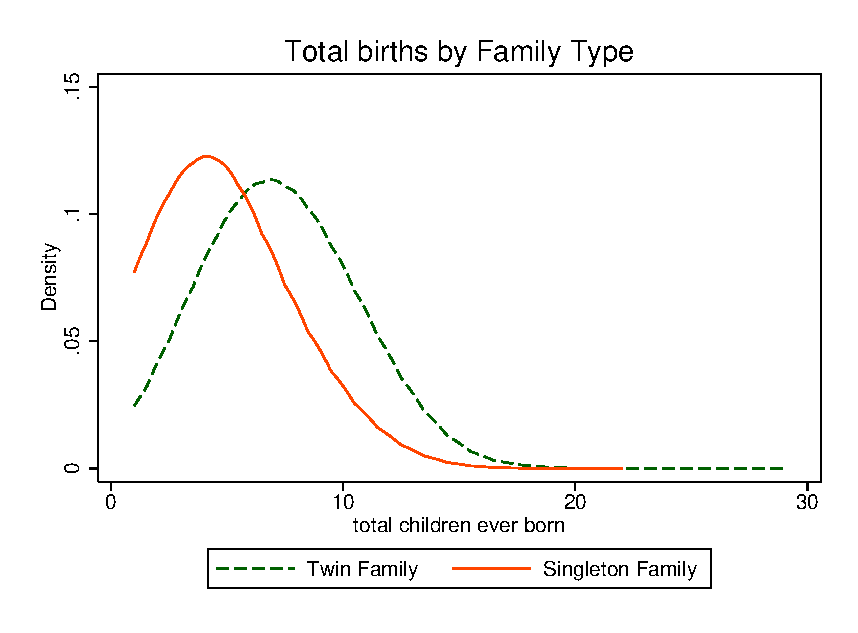
\includegraphics[scale=0.75]{./figures/famsize.eps}
\end{figure}
}

\frame{\frametitle{Twins Are More Likely to Occur at Higher Birth Orders}
\begin{figure}[htpb!]
\centering
  %\caption{Total births by Family Type}
  %\label{TWINfig:famsize}
  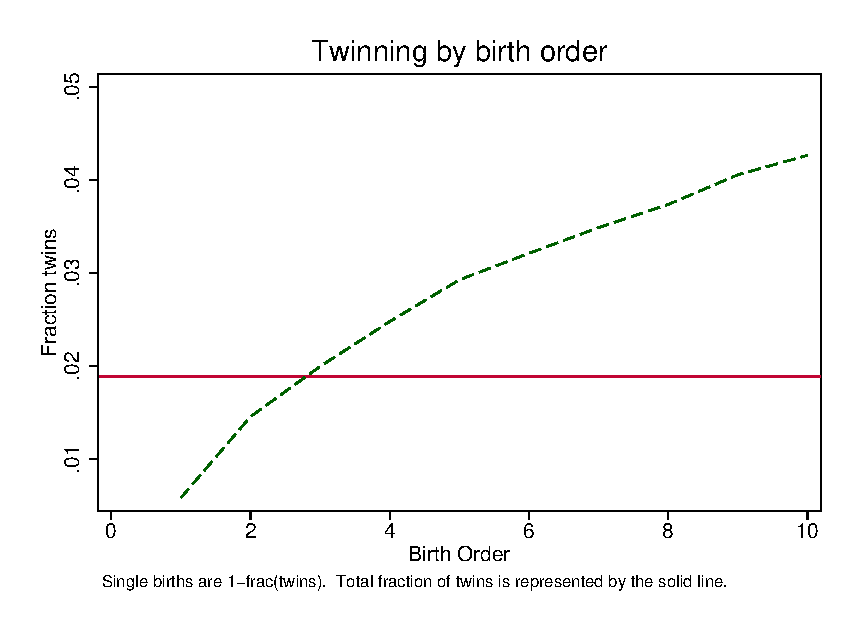
\includegraphics[scale=0.75]{./figures/twinbybord.eps}
\end{figure}
}


\section{Results}
\subsection{OLS Estimates}
\frame{\frametitle{OLS Estimates}
\begin{itemize}
\item OLS estimates will over-estimate the size of the trade-off if fertility and investments in children are simultaneously determined
\item Similarly, parental heterogeneity by fertility level will bias estimates (Qian, 2005)
\item Can use the Altonji-Taber statistic to assess the chance that the estimated trade-off is entirely spurrious
\end{itemize}
}

\frame{\frametitle{OLS Estimates}
Adding controls for predictors of twin birth diminishes the estimated trade-off
\begin{landscape}\begin{table}[!htbp] \centering 
\caption{OLS Estimates of the Q-Q Trade-off} 
 \vspace{4mm}\label{TWINtab:OLS} 
\begin{tabular}{lcccccc} \toprule \toprule 
&Base&+&+&Desired&Altonji&Altonji\\
&Controls&Socioec&Health&&Ratio 1&Ratio 2\\\midrule
\textsc{Panel A: All Countries}&&&&&&\\
Fertility &-0.115***&-0.0777***&-0.0751***&-0.0717***&2.083&1.882\\
&(0.000815)&(0.000776)&(0.000771)&(0.000838)&&\\
Fertility$\times$desire&&&&-0.00558***&&\\
&&&&(0.000495)&&\\
&&&&&&\\
Observations &1,334,874&1,334,874&1,334,874&1,334,874&&\\
R$^2$&0.094&0.161&0.167&0.168&&\\\midrule
\textsc{Panel B: Low Income}&&&&&&\\
Fertility &-0.110***&-0.0734***&-0.0712***&-0.0668***&2.005&1.835\\
&(0.00106)&(0.000988)&(0.000975)&(0.00107)&&\\
Fertility$\times$desire&&&&-0.00674***&&\\
&&&&(0.000608)&&\\
&&&&&&\\
Observations &831,476&831,476&831,476&831,476&&\\
R$^2$&0.091&0.171&0.181&0.182&&\\\midrule
\textsc{Panel C: Middle Income}&&&&&&\\
Fertility &-0.125***&-0.0875***&-0.0854***&-0.0839***&2.333&2.157\\
&(0.00128)&(0.00126)&(0.00126)&(0.00134)&&\\
Fertility$\times$desire&&&&-0.00266***&&\\
&&&&(0.000846)&&\\
&&&&&&\\
Observations &503,398&503,398&503,398&503,398&&\\
R$^2$&0.106&0.154&0.156&0.156&&\\\hline\hline
\multicolumn{7}{p{15.8cm}}{\begin{footnotesize}\textsc{Notes:} Base controls consist of child gender, mother's age and age squared mother's age at first birth, child age, country, and year of birth dummies.  Socioeconomic augments `Base' to include mother's education and education squared, and Health includes mother's height and BMI. ``Desire'' takes 1 if the child is born before the family reaches it's desired size, and 0 if the child is born after the desired size is reached. The \citet{Altonjietal2005} ratio determines how important unobservable factors must be compared with included observables to imply that the true effect of fertilty on educational attainment is equal to zero.  Ratio 1 compares no controls to socioeconomic controls, while ratio 2 compares no controls to socioeconomic and health controls. Standard errors are clustered at the level of the mother.
$^{*}$p$<$0.1; $^{**}$p$<$0.05; $^{***}$p$<$0.01\end{footnotesize}}\\  
\bottomrule \normalsize\end{tabular}\end{table}\end{landscape} 

}

\frame{\frametitle{Altonji, Elder, Taber 2005, extension in Bellows and Miguel 2009}
\[
schooling = \beta fertility+ X\delta + e
\]
\begin{itemize}
\item Fertility is endogenous and instrumented by twins and $X$ is a vector of relevant controls, conditional upon which twins are a valid instrument.
\item \textcolor{red}{Suppose we observe only a random sub-set of $X$.}
\item Assume that the observed and unobserved components of X are correlated and selection on unobservables is similar to selection on observables.
\item Compute the ratio of $\beta_c/(\beta_n-\beta_c)$ . A large ratio (given by controls not changing $\beta$ much) suggests it is implausible that unobservables can explain away the estimated impact.
\end{itemize}
}

\frame{\frametitle{Our Estimates}
\begin{itemize}
\item The Altonji et al.\ statistic computed from OLS estimates with and without controls for twin predictors is $\sim$2.
\item So for unobservables to explain the OLS coef (-0.12), the variation explained by unobservables would need to be about twice as large as the variation that is explained by the covariates included in our specification.
\end{itemize}
}

\subsection{IV Estimates}
\frame{\frametitle{IV Estimates}
\begin{itemize}
\item Fertility is instrumented with twin-birth
\item Under-estimate trade-off if twin-birth is endogenous
\item Demonstrate with observables and Conley bounds
\end{itemize}
}

\frame{\frametitle{The incidence of twins predicts an increase in fertility of $\sim$0.8 children (Similar if completed fertility)}
\begin{landscape}\begin{table}[htpb!]\caption{First Stage Results} 
\label{TWINtab:FS}\begin{center}\begin{tabular}{lcccp{2mm}cccp{2mm}ccc}
\toprule \toprule 
&\multicolumn{3}{c}{2+}&&\multicolumn{3}{c}{3+}&&\multicolumn{3}{c}{4+}\\ \cmidrule(r){2-4} \cmidrule(r){6-8} \cmidrule(r){10-12} 
\textsc{Fertility}&Base&+H&+S\&H&&Base&+H&+S\&H&&Base&+H&+S\&H\\ \midrule 
\begin{footnotesize}\end{footnotesize}& 
\begin{footnotesize}\end{footnotesize}& 
\begin{footnotesize}\end{footnotesize}& 
\begin{footnotesize}\end{footnotesize}& 
\begin{footnotesize}\end{footnotesize}& 
\begin{footnotesize}\end{footnotesize}& 
\begin{footnotesize}\end{footnotesize}& 
\begin{footnotesize}\end{footnotesize}& 
\begin{footnotesize}\end{footnotesize}& 
\begin{footnotesize}\end{footnotesize}\\ 
\multicolumn{12}{l}{\textbf{All}}\\ 
Twin&0.776***&0.821***&0.822***&&0.794***&0.827***&0.826***&&0.840***&0.859***&0.861***\\
&(0.031)&(0.029)&(0.028)&&(0.027)&(0.027)&(0.026)&&(0.027)&(0.027)&(0.026)\\
\begin{footnotesize}\end{footnotesize}&\begin{footnotesize}\end{footnotesize}&\begin{footnotesize}\end{footnotesize}&\begin{footnotesize}\end{footnotesize}&\begin{footnotesize}\end{footnotesize}&\begin{footnotesize}\end{footnotesize}&\begin{footnotesize}\end{footnotesize}&\begin{footnotesize}\end{footnotesize}&\begin{footnotesize}\end{footnotesize}&\begin{footnotesize}\end{footnotesize}&\begin{footnotesize}\end{footnotesize}&\begin{footnotesize}\end{footnotesize}\\Observations&249536&249536&249536&&249536&249536&249536&&249536&249536&249536\\
\begin{footnotesize}\end{footnotesize}&\begin{footnotesize}\end{footnotesize}&\begin{footnotesize}\end{footnotesize}&\begin{footnotesize}\end{footnotesize}&\begin{footnotesize}\end{footnotesize}&\begin{footnotesize}\end{footnotesize}&\begin{footnotesize}\end{footnotesize}&\begin{footnotesize}\end{footnotesize}&\begin{footnotesize}\end{footnotesize}&\begin{footnotesize}\end{footnotesize}&\begin{footnotesize}\end{footnotesize}&\begin{footnotesize}\end{footnotesize}\\\multicolumn{12}{l}{\textbf{Low-Income}}\\ 
Twin&0.826***&0.853***&0.848***&&0.810***&0.828***&0.834***&&0.867***&0.873***&0.869***\\
&(0.038)&(0.038)&(0.037)&&(0.033)&(0.033)&(0.032)&&(0.033)&(0.033)&(0.033)\\
\begin{footnotesize}\end{footnotesize}&\begin{footnotesize}\end{footnotesize}&\begin{footnotesize}\end{footnotesize}&\begin{footnotesize}\end{footnotesize}&\begin{footnotesize}\end{footnotesize}&\begin{footnotesize}\end{footnotesize}&\begin{footnotesize}\end{footnotesize}&\begin{footnotesize}\end{footnotesize}&\begin{footnotesize}\end{footnotesize}&\begin{footnotesize}\end{footnotesize}&\begin{footnotesize}\end{footnotesize}&\begin{footnotesize}\end{footnotesize}\\Observations&149602&149602&149602&&149602&149602&149602&&149602&149602&149602\\
\begin{footnotesize}\end{footnotesize}&\begin{footnotesize}\end{footnotesize}&\begin{footnotesize}\end{footnotesize}&\begin{footnotesize}\end{footnotesize}&\begin{footnotesize}\end{footnotesize}&\begin{footnotesize}\end{footnotesize}&\begin{footnotesize}\end{footnotesize}&\begin{footnotesize}\end{footnotesize}&\begin{footnotesize}\end{footnotesize}&\begin{footnotesize}\end{footnotesize}&\begin{footnotesize}\end{footnotesize}&\begin{footnotesize}\end{footnotesize}\\\multicolumn{12}{l}{\textbf{Middle-Income}}\\ 
Twin&0.718***&0.774***&0.784***&&0.757***&0.817***&0.801***&&0.783***&0.831***&0.839***\\
&(0.050)&(0.045)&(0.043)&&(0.046)&(0.045)&(0.043)&&(0.047)&(0.044)&(0.042)\\
\begin{footnotesize}\end{footnotesize}&\begin{footnotesize}\end{footnotesize}&\begin{footnotesize}\end{footnotesize}&\begin{footnotesize}\end{footnotesize}&\begin{footnotesize}\end{footnotesize}&\begin{footnotesize}\end{footnotesize}&\begin{footnotesize}\end{footnotesize}&\begin{footnotesize}\end{footnotesize}&\begin{footnotesize}\end{footnotesize}&\begin{footnotesize}\end{footnotesize}&\begin{footnotesize}\end{footnotesize}&\begin{footnotesize}\end{footnotesize}\\Observations&99934&99934&99934&&99934&99934&99934&&99934&99934&99934\\
\begin{footnotesize}\end{footnotesize}&\begin{footnotesize}\end{footnotesize}&\begin{footnotesize}\end{footnotesize}&\begin{footnotesize}\end{footnotesize}&\begin{footnotesize}\end{footnotesize}&\begin{footnotesize}\end{footnotesize}&\begin{footnotesize}\end{footnotesize}&\begin{footnotesize}\end{footnotesize}&\begin{footnotesize}\end{footnotesize}&\begin{footnotesize}\end{footnotesize}&\begin{footnotesize}\end{footnotesize}&\begin{footnotesize}\end{footnotesize}\\\multicolumn{12}{l}{\textbf{Adjusted Fertility}}\\ 
Twin&0.354***&0.393***&0.395***&&0.403***&0.428***&0.427***&&0.453***&0.467***&0.468***\\
&(0.028)&(0.028)&(0.028)&&(0.026)&(0.026)&(0.026)&&(0.027)&(0.027)&(0.027)\\
\begin{footnotesize}\end{footnotesize}&\begin{footnotesize}\end{footnotesize}&\begin{footnotesize}\end{footnotesize}&\begin{footnotesize}\end{footnotesize}&\begin{footnotesize}\end{footnotesize}&\begin{footnotesize}\end{footnotesize}&\begin{footnotesize}\end{footnotesize}&\begin{footnotesize}\end{footnotesize}&\begin{footnotesize}\end{footnotesize}&\begin{footnotesize}\end{footnotesize}&\begin{footnotesize}\end{footnotesize}&\begin{footnotesize}\end{footnotesize}\\Observations&249505&249505&249505&&249505&249505&249505&&249505&249505&249505\\
\begin{footnotesize}\end{footnotesize}&\begin{footnotesize}\end{footnotesize}&\begin{footnotesize}\end{footnotesize}&\begin{footnotesize}\end{footnotesize}&\begin{footnotesize}\end{footnotesize}&\begin{footnotesize}\end{footnotesize}&\begin{footnotesize}\end{footnotesize}&\begin{footnotesize}\end{footnotesize}&\begin{footnotesize}\end{footnotesize}&\begin{footnotesize}\end{footnotesize}&\begin{footnotesize}\end{footnotesize}&\begin{footnotesize}\end{footnotesize}\\\multicolumn{12}{l}{\textbf{Twins and Pre-Twins}}\\ 
Twin&0.727***&0.782***&0.788***&&0.809***&0.828***&0.832***&&0.853***&0.855***&0.859***\\
&(0.027)&(0.025)&(0.025)&&(0.027)&(0.026)&(0.026)&&(0.027)&(0.025)&(0.025)\\
\begin{footnotesize}\end{footnotesize}&\begin{footnotesize}\end{footnotesize}&\begin{footnotesize}\end{footnotesize}&\begin{footnotesize}\end{footnotesize}&\begin{footnotesize}\end{footnotesize}&\begin{footnotesize}\end{footnotesize}&\begin{footnotesize}\end{footnotesize}&\begin{footnotesize}\end{footnotesize}&\begin{footnotesize}\end{footnotesize}&\begin{footnotesize}\end{footnotesize}&\begin{footnotesize}\end{footnotesize}&\begin{footnotesize}\end{footnotesize}\\Observations&488815&488815&488815&&488815&488815&488815&&488815&488815&488815\\

\midrule\multicolumn{12}{p{19.2cm}}{\begin{footnotesize}\textsc{Notes:} Each cell represents the coefficient from the first-stage of a two-stage regression.  The first-stage represents the effect of twinning at parity $N$ on total fertility where $N$ is 2, 3 or 4 for 2+, 3+ and 4+ groups respectively.  The 2+ group includes all first borns in families with at least 2 births, the 3+ group includes first and second borns in families with at least 3 births, and the 4+ group includes all first to third borns in families with at least four births.  In each regressions the sample is made up of all children aged between 6-18 years from families in the DHS who fulfill these birth order conditions.  Controls in each case are identical to those described in table \ref{TWINtab:IVAll}.  Standard errors are clustered at the level of the mother.$^{*}$p$<$0.1; $^{**}$p$<$0.05; $^{***}$p$<$0.01 
\end{footnotesize}} \\ \bottomrule 
\end{tabular}\end{center}\end{table}\end{landscape}
}

\frame{
\begin{table}[htpb!]\caption{Principal IV Results}
\label{TWINtab:IVAll}
\begin{center}\scalebox{0.55}{
\begin{tabular}{lcccp{2mm}cccp{2mm}ccc}
\toprule \toprule 
&\multicolumn{3}{c}{2+}&&\multicolumn{3}{c}{3+}&&\multicolumn{3}{c}{4+}\\ \cmidrule(r){2-4} \cmidrule(r){6-8} \cmidrule(r){10-12} 
\textsc{School Z-Score}&Base&+H&+S\&H&&Base&+H&+S\&H&&Base&+H&+S\&H\\ \midrule 
\begin{footnotesize}\end{footnotesize}& 
\begin{footnotesize}\end{footnotesize}& 
\begin{footnotesize}\end{footnotesize}& 
\begin{footnotesize}\end{footnotesize}& 
\begin{footnotesize}\end{footnotesize}& 
\begin{footnotesize}\end{footnotesize}& 
\begin{footnotesize}\end{footnotesize}& 
\begin{footnotesize}\end{footnotesize}& 
\begin{footnotesize}\end{footnotesize}& 
\begin{footnotesize}\end{footnotesize}& 
\begin{footnotesize}\end{footnotesize}& 
\begin{footnotesize}\end{footnotesize}\\ 
\multicolumn{12}{l}{\textbf{All}}\\ 
Fertility&0.006&-0.026&-0.026&&-0.004&-0.036&-0.038*&&-0.017&-0.036&-0.035*\\
&(0.029)&(0.027)&(0.026)&&(0.024)&(0.022)&(0.021)&&(0.025)&(0.023)&(0.021)\\
\begin{footnotesize}\end{footnotesize}&\begin{footnotesize}\end{footnotesize}&\begin{footnotesize}\end{footnotesize}&\begin{footnotesize}\end{footnotesize}&\begin{footnotesize}\end{footnotesize}&\begin{footnotesize}\end{footnotesize}&\begin{footnotesize}\end{footnotesize}&\begin{footnotesize}\end{footnotesize}&\begin{footnotesize}\end{footnotesize}&\begin{footnotesize}\end{footnotesize}&\begin{footnotesize}\end{footnotesize}&\begin{footnotesize}\end{footnotesize}\\Observations&249536&249536&249536&&375987&375987&375987&&385389&385389&385389\\
\multicolumn{12}{l}{\textbf{Low-Income}}\\ 
Fertility&0.035&0.008&0.012&&0.016&-0.016&-0.027&&-0.011&-0.031&-0.024\\
&(0.034)&(0.032)&(0.031)&&(0.030)&(0.028)&(0.026)&&(0.029)&(0.027)&(0.025)\\
\begin{footnotesize}\end{footnotesize}&\begin{footnotesize}\end{footnotesize}&\begin{footnotesize}\end{footnotesize}&\begin{footnotesize}\end{footnotesize}&\begin{footnotesize}\end{footnotesize}&\begin{footnotesize}\end{footnotesize}&\begin{footnotesize}\end{footnotesize}&\begin{footnotesize}\end{footnotesize}&\begin{footnotesize}\end{footnotesize}&\begin{footnotesize}\end{footnotesize}\\Observations&149602&149602&149602&&232371&232371&232371&&246622&246622&246622\\
\multicolumn{12}{l}{\textbf{Middle-Income}}\\ 
Fertility&-0.065&-0.087*&-0.093**&&-0.046&-0.079**&-0.067*&&-0.027&-0.048&-0.054\\
&(0.053)&(0.049)&(0.047)&&(0.040)&(0.036)&(0.035)&&(0.043)&(0.040)&(0.037)\\
\begin{footnotesize}\end{footnotesize}&\begin{footnotesize}\end{footnotesize}&\begin{footnotesize}\end{footnotesize}&\begin{footnotesize}\end{footnotesize}&\begin{footnotesize}\end{footnotesize}&\begin{footnotesize}\end{footnotesize}&\begin{footnotesize}\end{footnotesize}&\begin{footnotesize}\end{footnotesize}&\begin{footnotesize}\end{footnotesize}&\begin{footnotesize}\end{footnotesize}\\Observations&99934&99934&99934&&143616&143616&143616&&138767&138767&138767\\
\multicolumn{12}{l}{\textbf{Adjusted Fertility}}\\ 
Fertility&0.017&-0.052&-0.055&&-0.013&-0.073*&-0.077*&&-0.033&-0.068&-0.066*\\
&(0.065)&(0.056)&(0.054)&&(0.047)&(0.043)&(0.040)&&(0.045)&(0.042)&(0.039)\\
\begin{footnotesize}\end{footnotesize}&\begin{footnotesize}\end{footnotesize}&\begin{footnotesize}\end{footnotesize}&\begin{footnotesize}\end{footnotesize}&\begin{footnotesize}\end{footnotesize}&\begin{footnotesize}\end{footnotesize}&\begin{footnotesize}\end{footnotesize}&\begin{footnotesize}\end{footnotesize}&\begin{footnotesize}\end{footnotesize}&\begin{footnotesize}\end{footnotesize}\\Observations&249505&249505&249505&&375957&375957&375957&&385363&385363&385363\\
\multicolumn{12}{l}{\textbf{Twins and Pre-Twins}}\\ 
Fertility&-0.021&-0.073***&-0.078***&&-0.019&-0.062***&-0.067***&&-0.018&-0.039**&-0.046**\\
&(0.024)&(0.021)&(0.020)&&(0.020)&(0.018)&(0.018)&&(0.021)&(0.019)&(0.018)\\
\begin{footnotesize}\end{footnotesize}&\begin{footnotesize}\end{footnotesize}&\begin{footnotesize}\end{footnotesize}&\begin{footnotesize}\end{footnotesize}&\begin{footnotesize}\end{footnotesize}&\begin{footnotesize}\end{footnotesize}&\begin{footnotesize}\end{footnotesize}&\begin{footnotesize}\end{footnotesize}&\begin{footnotesize}\end{footnotesize}&\begin{footnotesize}\end{footnotesize}\\Observations&488815&488815&488815&&563177&563177&563177&&523197&523197&523197\\
\bottomrule
\end{tabular}}\end{center}\end{table}

}

\frame{\frametitle{IV Results by Gender}
\begin{table}[htpb!]\caption{Q-Q IV Estimates by Gender} 
\label{TWINtab:gend}\begin{center}\begin{tabular}{lcccccccc}
\toprule \toprule 
&\multicolumn{4}{c}{Females}&\multicolumn{4}{c}{Males}\\ 
\cmidrule(r){2-5} \cmidrule(r){6-9} 
&Base&Socioec&Health&Obs.&Base&Socioec&Health&Obs. \\ \midrule 
\begin{footnotesize}\end{footnotesize}&\begin{footnotesize}\end{footnotesize}&\begin{footnotesize}\end{footnotesize}&\begin{footnotesize}\end{footnotesize}&\begin{footnotesize}\end{footnotesize}&\begin{footnotesize}\end{footnotesize}&\\Two Plus &0.005&-0.039&-0.037&122,414&0.010&-0.010&-0.015&127,122\\
&(0.043)&(0.039)&(0.038)&&(0.040)&(0.038)&(0.036)&\\
\begin{footnotesize}\end{footnotesize}&\begin{footnotesize}\end{footnotesize}&\begin{footnotesize}\end{footnotesize}&\begin{footnotesize}\end{footnotesize}&\begin{footnotesize}\end{footnotesize}&\begin{footnotesize}\end{footnotesize}&\\Three Plus &-0.024&-0.056*&-0.052*&187,098&0.016&-0.015&-0.022&188,889\\
&(0.033)&(0.030)&(0.029)&&(0.030)&(0.028)&(0.027)&\\
\begin{footnotesize}\end{footnotesize}&\begin{footnotesize}\end{footnotesize}&\begin{footnotesize}\end{footnotesize}&\begin{footnotesize}\end{footnotesize}&\begin{footnotesize}\end{footnotesize}&\begin{footnotesize}\end{footnotesize}&\\Four Plus &-0.029&-0.052*&-0.053**&192,714&-0.005&-0.020&-0.018&192,675\\
&(0.032)&(0.029)&(0.027)&&(0.030)&(0.028)&(0.027)&\\
\midrule\multicolumn{9}{p{14.2cm}}{\begin{footnotesize}\textsc{Notes:} Female or male refers to the gender of the index child of the regression. 
All regressions include full controls including socioeconomic and maternal health variables.  The full lis of controls are available in 
the notes to table \ref{TWINtab:IVAll}.  Full IV results for male and female children are presented in table \ref{TWINtab:IVgend}. Standard errors are clustered 
 by mother.$^{*}$p$<$0.1; $^{**}$p$<$0.05; $^{***}$p$<$0.01
\end{footnotesize}} \\ \bottomrule 
\end{tabular}\end{center}\end{table}
}

\frame{\frametitle{Taking Stock: OLS vs.\ IV}
\begin{itemize}
\item \textcolor{red}{First stage} indicates twin birth is a powerful instrument. 
\item Conditional upon available SES and health controls, the OLS estimate is $-0.08^{*}$ (parity pooled). 
\begin{itemize}
\item OLS estimates are smaller in absolute terms conditional upon mother characteristics. Consistent with high fertility women tending to have lower tastes for education.
\end{itemize}
\item IV estimates are $-0.04^{*}$ (3+, all) to $-0.06^{*}$ (3+, middle income). 
\begin{itemize}
\item IV estimates grow larger in absolute terms conditional upon mother characteristics: consistent with our hypothesis. 
\item Trade-off emerges in middle-income countries at 2+ and in middle-inc and pooled sample at 3+ and upwards. 
\end{itemize}
\end{itemize}
}


\frame{\frametitle{Taking Stock: IV Results}
\begin{itemize}
\item Trade-off is clearer in middle-income countries
\begin{itemize}
\item Institutional constraints may limit investments in quality in low-income countries.
\end{itemize}
\item Trade-off is smaller in 4+ and 5+ samples
\begin{itemize}
\item These high-fertility families may have different preferences, valuing quality less
\end{itemize}
\item Trade-off is larger and only significant for girls
\begin{itemize}
\item Consistent with girl ``quality'' being more of a luxury
\end{itemize}
\item In 4+ and 5+ samples there is evidence of the trade off being driven by (larger) in families where twins take fertility over the desired level- consistent with our hypothesis
\item Including twins with pre-twins in the sample strengthens the trade-off: they are not fully compensated.
\end{itemize}
}

\subsection{Bounds}
\frame{\frametitle{Bounds}
\begin{itemize}
\item Estimate a $\beta$ interval for a plausible range of $\gamma\neq 0$
\item Can bound in two ways: 
\begin{itemize}
\item OLS versus IV
\item Loosen the strong assumption of instrumental validity
\end{itemize}
\end{itemize}
}

\frame{\frametitle{OLS and IV bound the tradeoff }
\begin{itemize}
\item High fertility women are \textcolor{red}{negatively selected}
\begin{itemize}
\item So controlling for fertility predictors weakens OLS estimates of the QQ tradeoff.
\end{itemize}
\item Women who are predisposed toward having twins are \textcolor{red}{positively selected}
\begin{itemize}
\item So controlling for predictors of twin birth strengthens IV estimates of the QQ tradeoff.
\end{itemize}
\item This allows us to treat OLS and IV estimates as bounds on the true parameter
\begin{itemize}
\item The caveat to this is that we will tend to under-estimate the lower bound (IV) because it is impossible to fully control for mother characteristics that determine fetal health and predict twinning.
\end{itemize}
\item Can thus tighten bounds (on both sides) by controlling for additional health and socioeconomic variables
\end{itemize}
}


\frame{\frametitle{Bounds derived on the premise of plausible exogeneity}
An alternative approach to inference for IV models with instruments whose validity is debatable.
\[
schooling = \beta fertility + \textcolor{red}{\gamma twins} + X\delta+ e
\]
\begin{itemize}
\item Relax the exclusion restriction that $\gamma=0$.
\item Plausible exogeneity corresponds to having prior information that $\gamma$ is near 0 but not exactly 0 (Conley et al.\ 2012)
\item The \textcolor{red}{2SLS estimator is less sensitive to violations of the exclusion restriction when the instrument is strong} (related, Bound, Jaeger, Baker 1995). Conley et al.\ are motivated by cases such as ours where the instrument is strong but may not be strictly exogenous.
\item Nevo and Rosen (2012) discuss a similar estimation strategy
\end{itemize}
}

\frame{\frametitle{The Procedure}
Conley et al. 2012 present four complementary inference strategies that use prior information about $\gamma$ to different extents. We implement two of these: union of confidence interval (UCI) and the local to zero approach (LTZ)
\vspace{4mm}
\begin{itemize}
\item We specify a set of plausible values for $\gamma$ and obtain interval estimates for $\beta$ conditional upon each.  Grid over 0 to 2$\hat\gamma$.
\item Taking the union of these interval estimates across values of $\gamma$ provides a conservative interval estimate for $\beta$.
\begin{itemize}
\item The plus is that we don’t need to specify a prior distribution for $\gamma$, just a range of plausible values.
\item The minus is that the estimated interval around $\beta$ may be wide
\end{itemize}
\item The LTZ approach views prior probabilities for $\gamma$ as analogous to objective probabilities in a 2-step DGP.  Here we must specificy a prior distribution.
\end{itemize}
}

\frame{\frametitle{Estimates of bounds:UCI and LTZ Approaches}
\begin{table}[htpb!]\caption{`Plausibly Exogenous' Bounds} 
\label{TWINtab:Conley}\begin{center}\begin{tabular}{lcccc}
\toprule \toprule 
&\multicolumn{2}{c}{UCI: $\gamma\in [0,\delta]$}&\multicolumn{2}{c}{LTZ: $\gamma \sim U(0,\delta)$}\\ 
\cmidrule(r){2-3} \cmidrule(r){4-5}
&Lower Bound&Upper Bound&Lower Bound&Upper Bound\\
Two Plus&-0.1860&0.0195&-0.1613&0.0011\\
Three Plus&-0.1710&0.0025&-0.1528&-0.0116\\
Four Plus&-0.1539&-0.0067&-0.1391&-0.0194\\
Five Plus&-0.1373&0.0277&-0.1215&0.0143\\
\midrule\multicolumn{5}{p{11.6cm}}{\begin{footnotesize}\textsc{Notes:} This table presents upper and lower bounds of a 95\% confidence interval for the effects of family size on (standardised) children's education attainment. These are estimated by the methodology of \citet{Conleyetal2012}  under various priors about the direct effect that being from a twin family has on educational outcomes ($\gamma$). In the UCI (union of confidence interval) approach, it is assumed the true $\gamma\in[0,\delta]$, while in the LTZ (local to zero) approach it is assumed that $\gamma\sim U(0,\delta)$.  In each case $\delta$ is estimated by including twinning in the first stage  equation and observing the effect size $\hat\gamma$.  Estimated $\hat\gamma$'s are (respectively for two plus to five plus):   0.1088, 0.0983, 0.0826, 0.0929.\end{footnotesize}}  
\\ \bottomrule \end{tabular}\end{center}\end{table} 

}


\frame{\frametitle{Estimates (3+) Assuming that $\gamma \sim U(0,\delta)$}
\begin{figure}[htpb!]
\centering
  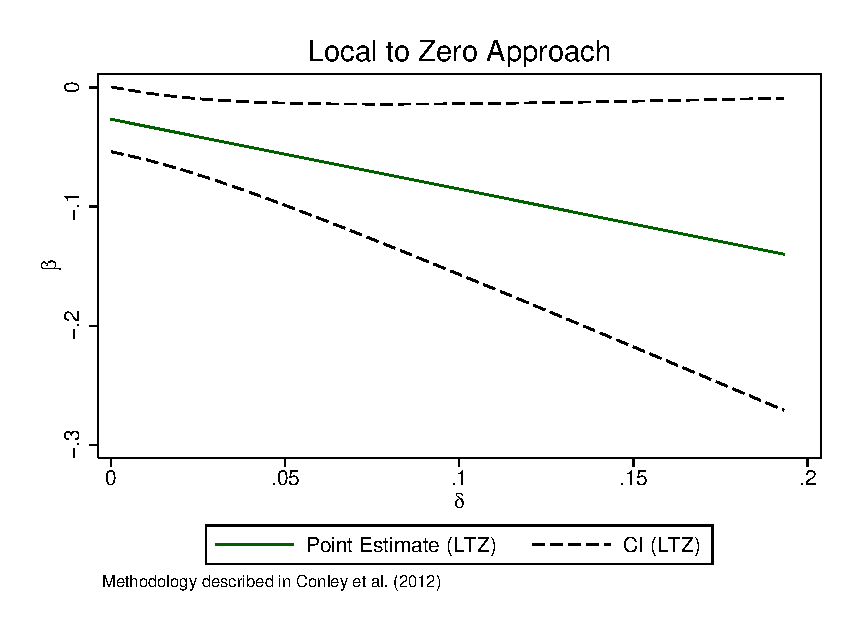
\includegraphics[scale=0.75]{./figures/LTZ_three.eps}
\end{figure}
}

\section{Conclusions}
\frame{\frametitle{Conclusions}
\begin{itemize}
\item Indicators of mother's health, education, wealth and age are significant predictors of twin birth.
\item As are positive behaviours during pregnancy
\item Families that at some date have a twin have significantly lower infant mortality rates prior to occurrence of twins (consistent with their being healthier).
\item Conditioning upon available twin predictors produces evidence of a tradeoff in IV ($\sim -0.04$ s.d.) and RF estimates.
\item Recognizing that twins are at best plausibly exogenous results in a QQ parameter interval with an upper bound of $\sim -0.15$ s.d. 
\item Significantly larger trade-off for middle income countries and for female children
\end{itemize}
}

\frame{
Thank you.
}

\frame{\frametitle{Estimates (2+) Assuming that $\gamma \sim U(0,\delta)$}
\begin{figure}[htpb!]
\centering
  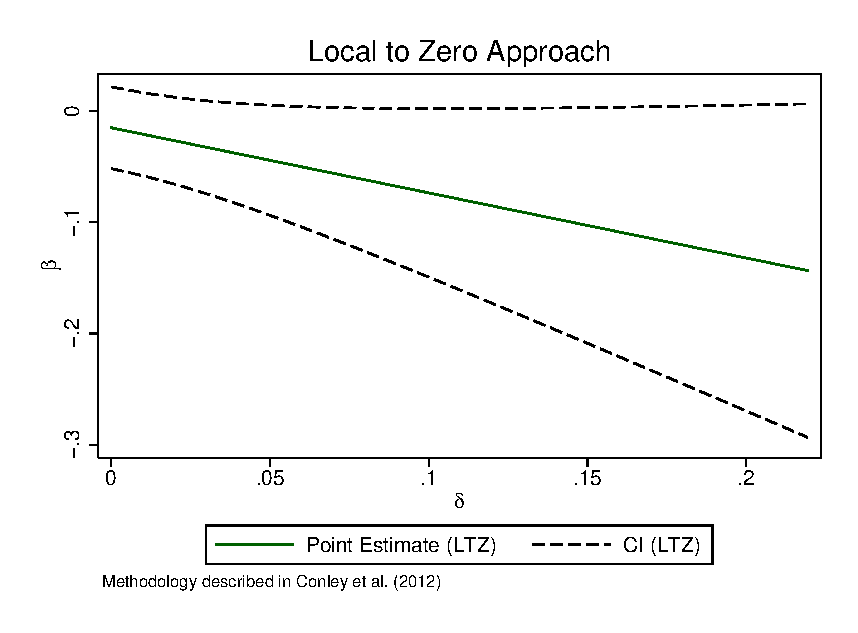
\includegraphics[scale=0.75]{./figures/LTZ_two.eps}
\end{figure}
}

\frame{\frametitle{Estimates (4+) Assuming that $\gamma \sim U(0,\delta)$}
\begin{figure}[htpb!]
\centering
  \includegraphics[scale=0.75]{./figures/LTZ_four.eps}
\end{figure}
}

\end{document}


%********************************************************************************
%********************************************************************************
%********************************************************************************
%********************************************************************************
%********************************************************************************
%********************************************************************************
%********************************************************************************
%********************************************************************************
%********************************************************************************
%********************************************************************************
